\documentclass[tikz,border=10pt]{standalone}
\usetikzlibrary{calc}
\begin{document}
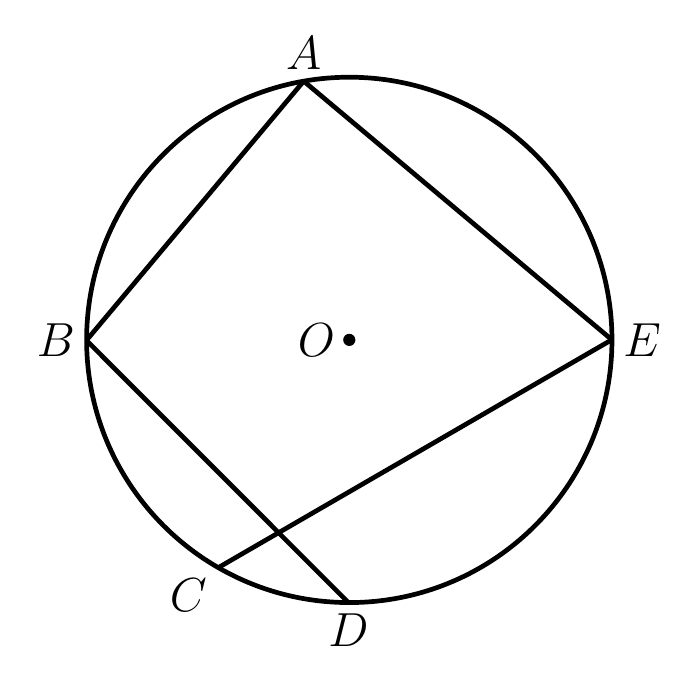
\begin{tikzpicture}[line width=1.7pt, line join=round]
  % Scale s = 0.02122 cm/px, origin at O (px 225.98, 220.25), y flipped
  \coordinate (O) at (0,0);
  \coordinate (A) at (-0.579,3.286);
  \coordinate (B) at (-3.338,-0.006);
  \coordinate (E) at (3.334,0.002);
  \coordinate (C) at (-1.663,-2.892);
  \coordinate (D) at (-0.011,-3.336);

  % Circle of radius 157.2 px
  \draw (O) circle[radius=3.336cm];

  % Chords (solid, endpoints at vertices)
  \draw (A) -- (B);
  \draw (A) -- (E);
  \draw (B) -- (D);
  \draw (E) -- (C);

  % Centre dot
  \fill (O) circle (2.2pt);

  % Labels (math italic, outside the circle)
  \node[font=\fontsize{17}{20.4}\selectfont, above] at (A) {$A$};
  \node[font=\fontsize{17}{20.4}\selectfont, left] at (B) {$B$};
  \node[font=\fontsize{17}{20.4}\selectfont, right] at (E) {$E$};
  \node[font=\fontsize{17}{20.4}\selectfont, below left] at (C) {$C$};
  \node[font=\fontsize{17}{20.4}\selectfont, below] at (D) {$D$};
  \node[font=\fontsize{17}{20.4}\selectfont, left, xshift=-1pt] at (O) {$O$};
\end{tikzpicture}
\end{document}